%===========================================
%             General INTRO
%===========================================
\chapter{General Introduction}

\begin{center}
    \textit{“There is still no clear resolution on the evolutionary forces responsible for the maintenance of variation. Estimates of critical quantities, such as the strength of selection and mutational parameters are still sufficiently fuzzy to allow advocates of any particular model to proclaim that it largely fits the data, and opponents to insist that it does not.”} \citet{Wals18}
\end{center}

\section{Models of the maintenance of standing genetic variation} 
The amount of standing genetic variation determines the rate at which a population can adapt to changes in the environment and determines a population’s evolutionary trajectory \citep{Land79, Hans08}. The loss of genetic variance, as in the case of small populations, leads to an increase in the mutation load and, subsequently, an increased risk of extinction \citep{Mull64, Lync90, Land94}. Through investigating the underlying mechanisms that create and maintain genetic variation we can gain better insight into the processes of evolution and population persistence. New alleles are introduced to a population through either mutation or migration, but ultimately all genetic variation is the result of mutation \citep{Falc96, John05}. Counterbalancing the influx of mutation are the processes of selection and drift. The magnitude of standing genetic variation is the outcome of the interaction among the opposing forces of mutation, selection and drift \citep{Fish30}. Despite knowing the primary processes involved in determining standing genetic variance, there still remains considerable uncertainty as to how genetic variance is maintained in natural populations \citep{Ture85, John05}. \par

The most basic model of the maintenance of genetic variance is the mutation-drift model, where the magnitude of genetic variation is a result of the gain of genetic variance through neutral mutation minus the variation lost due to drift \citep{Fran80, Bart90}. Genetic drift is the random sampling of alleles each generation, with the random sample likely to differ more from the true allele frequency in small populations \citep{Land76}. At mutation-drift equilibrium, standing genetic variance is predicted to be equal to the mutational variance scaled by the effective population size ($N_e$) (\citep{Lync86}. When mutation-drift models are parameterised with known estimates of mutational variance and $N_e$, they overpredict the magnitude of standing genetic variance \citep{John05, Wals18, McGu15}. Two independent lines of evidence suggest that mutation-drift balance alone cannot account for standing genetic variance and therefore lead to the expectation that selection will be an essential process determining the magnitude of genetic variation in populations. Most mutations with detectable phenotypic effects have deleterious effects on fitness, suggesting that mutations are typically not neutral \citep{Kond92, Hall09}. Moreover, estimates of selection acting on a wide range of traits in natural populations suggest that many traits are under directional selection \citep{King01, King12}.\par  

Balancing selection and stabilising selection are the two primary modes of selection included in models of the maintenance of genetic variation in quantitative traits. Although balancing selection might account for the maintenance of genetic variance in some specific cases, there is little support for this as a general mechanism \citep{Bart90, John05, Hedr12}. Mutation-stabilising selection balance (MSB) is a more generally applicable explanation of the maintenance of genetic variance, where, at equilibrium, new mutant alleles arise at the same rate that selection removes alleles from the population \citep{Trot01, John05, Zhan05}. There are many models of MSB, varying in the assumptions that they make about the genetic architecture of fitness or the focal traits, and about the plausible parameter values considered (e.g. \citealt{Latt70, Land75, Ture85, Keig88, Burg89, Kond92, Houl96, John05, Wals18}). The magnitude of genetic variance underlying a specific phenotype is contingent on the number of loci governing the phenotype, the distribution of phenotypic effects of alleles at those loci, and the frequency of alleles \citep{Ture88}. These details are generally unknown, but the quantitative genetic summaries of this information can generate insights into how genetic variation is maintained \citep{John05}.\par

Although mutation-selection balance models account for selection, they have consistently failed to explain the magnitude of observed standing genetic variance. Early MSB models assumed direct stabilising selection on a focal trait, that at each locus there is an infinite number of alleles and selection follows a Gaussian function. These models required extremely high mutation rates, well outside values observed from empirical studies \citep{Land75, Ture84}. Real stabilising selection models also assumed large proportions of mutations were beneficial, which contradicts the view that most mutations are deleterious \citep{Kond92}. A multivariate extension of stabilising selection models incorporates apparent stabilising selection, where mutations have a direct effect on a neutral focal trait and a deleterious pleiotropic effect on fitness \citep{Ture85, Bart90, Zhan03}. These types of models included deleterious properties of mutations but failed to simultaneously account for levels of segregating variation and strength of selection that appear to be operating on traits \citep{John05}. In pure pleiotropy models, genetic variation is assumed to be maintained either by overdominant effects on fitness or deleterious mutations that are in mutation-selection equilibrium \citep{John05}. The apparent shortcoming of these models occurs when $N_e$ approaches infinity, so does the estimates of standing genetic variance. Thus, mutation heritability tends toward one as $N_e$ increases \citep{Caba94}. Estimates of stabilising selection from the pure pleiotropy model are much weaker than observed stabilising selection, another limitation of these types models \citep{Wals18}. The last group of models are the joint effect models, which allows direct stabilising selection and drift to jointly act on mutants with deleterious pleiotropic fitness effects that affect multiple traits \citep{Zhan02}. When empirical values are considered in a joint effect model, it predicts high heritabilities and stabilizing selection, with small mutation rates \citep{Zhan02}. No model to date has been successful in describing the level of observed standing genetic variance, given the empirical estimates of mutational variance and selection \citep{John05, Houl17}.\par    

\section{Empirical estimates of mutational variance and selection strength} 
Understanding of the maintenance of genetic variance ($V_G$) in natural populations lies in understanding the increase in genetic variance caused by new mutations introduced each generation, the mutational variance ($V_M$), and the strength of selection ($s$) acting against new mutations.  Across many models of MSB, $V_M$ and $s$ are the two main parameters, where the underlying expectation is that higher $V_G$ results from either high $V_M$ or reduced $s$ \citep{Lync99}. One difficulty with assessing whether MSB models can reconcile observed levels of these parameters lies with the estimation of the parameters themselves \citep{Wals18}. \par

The most common method to estimate $V_M$ is to use a divergence experiment based on replicate lines derived from a single genetically homogeneous ancestral population, referred to as a mutation accumulation (MA) experiment \citep{Muka64, John05, Hall09}. Because replicate lines begin as genetically homogenous copies (at least in principle), any genetic variation between them is the result of spontaneous mutations arising and fixing independently in each line \citep{Hall09}. MA lines are kept at small effective population sizes (e.g., a single individual in clonal taxa or brother-sister pairs in sexually reproducing taxa) such that the fates of new mutations are determined by random drift \citep{Lync98}. The MA approach has been applied in a range of taxa including crop plants, microorganisms, insects and mice \citep{Houl96, Lync99}. To compare $V_M$ among diverse taxa and trait types, estimates are standardised, either against the environmental variance ($V_E$) to give the mutational heritability ($h_M^2$) or against the trait mean to give the mutational co-efficient of variation ($CV_M$) \citep{Houl96, Hall09}. Estimates of mutational heritabilities typically range between 0.001 to 0.01 and are typically higher for morphological traits ($\sim0.0025$) than life history traits \citep[$\sim0.0013$][]{Lync99}. Conversely, $CV_M$ measures for life history traits ($\sim0.019$, averaged across studies taken from \citealt{Houl96, Hall09}), are generally higher than morphological traits ($\sim0.004$, averaged from \citealt{Houl96}). \par

The difference between morphological and life history traits for $h_M^2$ and $CV_M$ is similar to observations for $V_G$ \citep{Houl92a}.  \citet{Houl92a} used published estimates of $V_G$ and $V_M$ to test several hypotheses explaining variation among trait types in their standing genetic variation. Generally, there is a strongly positive relationship between $V_G$ and $V_M$ (see Figure~\ref{fig:CvaCvm}), suggesting that mutation is the main process in maintaining standing genetic variance. Life history traits, including fecundity, longevity and viability had higher estimates for $V_M$, and $V_G$. Life history traits are expected to be determined by more loci and consequently the genetic target for mutation is expected to be larger \citep{Houl98}. Despite the intuitive expectation that selection plays a major role in determining the magnitude of standing genetic variation, the available empirical evidence suggests that mutational variation might be the major determining factor. \par

There are several different empirical approaches that have been taken to determine the selection acting on new mutations. Firstly, MA studies can provide information on selection by considering how mean fitness changes in the absence of selection. Such studies have typically reported declines in fitness, indicating that most new mutations have deleterious effects on fitness \citep{Hall09}. The average change in mean fitness per generation (\( \Delta M \)) is approximately 0.36\% \citep{Hall09}. Beneficial mutations have rarely been found in MA experiments and when detected typically occur at a much lower rate than deleterious mutations \citep{Jose04}. Surprisingly, \citet{Shaw00} demonstrated a nonsignificant \( \Delta M \)$<1$\% in \textit{Arabidopsis thaliana}, concluding that 50\% of the mutations were advantageous to fitness; however, this has been attributed to insufficient generations (17) and a bias in the underlying distributions of the model used to estimate \( \Delta M \) \citep{Keig03}. The majority of evidence suggests that mutations will be under selection, however, there is little information on the variation in the strength of selection acting on different trait types. To understand the variation in the magnitude of $V_G$, the contribution of variation in the strength of selection must be better characterised. \par

Mutation generally does not change trait mean of non-fitness traits, suggesting that mutations typically have an unbiased effect on traits other than fitness \citep{John05}. For wing traits of \textit{D. melanogaster}, \citet{Sant92} found no mutational bias in wing length and width, but in a subset of eight lines, with the greatest fitness changes, there was a consistent change in shape mean in the same direction. Similarly, \citet{McGu13} found no overall mutational bias on wing shape or size, but found that lines with larger size were more likely to go extinct earlier, suggesting that mutations increasing size typically decreased fitness. The pleiotropy class of MSB models require mutations to have deleterious effects on fitness but unbiased effects on non-fitness traits \citep{Keig90, Wals18}. Thus, a lack of change in morphological trait mean under MA experiments does not directly infer that new mutations affecting these traits are not under selection to remove them from the population. \par
 
A second approach used to gain insight into the strength of selection from MA experiments is to indirectly infer the strength of selection by comparing the magnitude of mutational and standing genetic variation \citep{Hall09}. The magnitude of selection can be calculated as the ratio of $V_M$ to $V_G$, where $s \approx V_M/V_G$ \citep{Bart90, char15}. Estimates of $s$ for fitness traits including egg-adult viability, fecundity and longevity have a median value of 0.021 \citep{Houl96}, although values as low as 0.01 or as high as 0.21 have been reported \citep{Muka72, Garc99}. The median estimate for morphological traits is (0.009) but a range of values (0.001 to 0.01) have been reported \citep{Houl96}. The largest values of $s$ for morphological traits are lower than for life history traits, consistent with the expectation of weaker selection on morphology \citep{Houl96}.  

The information that we have on the median strength of selection might not be informative of how effective selection is in natural populations if the distribution around that median value is skewed. Although it is widely accepted that the distribution of mutational effects on fitness is not centred on zero, the underlying shape of the mutational-effect distribution remains uncertain. The distribution of fitness effects of new mutations has long been considered strongly leptokurtic such that most mutations have weak effects while only some mutations have strong effects \citep{Kimu65, Robe67}. If the distribution of mutations is strongly leptokurtic, this suggests that selection will be less effective at removing the small effect mutations and that selection might typically be weaker than the median value suggests. However, the prediction of a leptokurtic distribution was not supported when estimates in the literature were reviewed; the distribution of mutational effects was more shifted toward a normal distribution than expected \citep{Hall09}. Despite most mutations having small deleterious effects, it is possible that under MA conditions a second class of relatively common and large effect mutations are also observed \citep{Hall09}. Further research is needed to determine the distribution of mutational effects, both on quantitative traits and on fitness per se.  \par

The efficacy of selection depends on $N_e$, such that mutations will be effectively neutral at selection coefficients of less than $1/2N_e$ \citep{Wrig31} and that the fate of mutations will be strongly affected by drift rather than deterministically removed by selection when $N_es<0.25$ \citep{Falc81}. Hence, manipulating the effective population size provides a third approach to understanding the selection acting on mutations. Only a few studies to date have manipulated the size of $N_e$ to determine strength of selection \citep{Este04, Sila07, Katj15}. \citet{Este04} used $N_e$ treatments ($N$ of 1, 5, and 25) in a high mutation rate strain of \textit{Caenorhabditis elegans} and found that mean fitness (productivity and survival) declined in smaller $N_e$ sizes while the variance among lines increased, consistent with the expectation that there was reduced selection on deleterious mutations in smaller populations. Also in \textit{C. elegans}, but considering naturally occurring mutations in a standard population, \citet{Katj15} reported strong fitness declines at $N_e = 1$ ($s <0.5$), but not in larger populations ($N_e = 5$ and 50; $s <0.1$ or 0.01). These values for $s$ are higher than the range of selection strength given by \citet{Houl96} ($0.009<s< 0.021$), for this reason it is surprising that the was no observed mutational effect on fitness. \citet{Katj15} compared change in treatment means to determine the distribution of effect, but did not estimate $V_M$, which would result in a direct estimate of selection. Both studies showed a decline in fitness in smaller $N_e$ sizes, but little to no change in larger treatments of $N_e$. This suggests that a few mutations of large effect are primarily responsible \citep{Este04, Hall09, Katj15}, where the distribution of selection coefficients are markedly different from the indirect estimates from previous studies \citep{Houl96}. Although \textit{C. elegans} can reproduce via sexual reproduction, these mutation accumulation experiments lines were maintained by self-fertilising hermaphrodites, which would have resulted in a different pattern of heterozygosity of new mutations compared with sexually reproducing taxa. \par

In natural, randomly mating populations, the fate of new mutations depends on the strength of selection acting on heterozygote fitness \citep{Simm77}. As a result, dominant mutations are removed from the population faster than equally deleterious recessive mutations. Observations on inbreeding depression indicate that many of the deleterious alleles segregating in natural populations have recessive effects on fitness \citep{Char87}. Direct empirical estimates of dominance coefficients suggest a relationship between the effect of a mutation on fitness and its dominance. On average, small effect mutations are partially recessive, while highly deleterious mutations are recessive \citep{Caba97, Hall09, Agra11}. However, estimates of dominance coefficients have been reported showing the full range from fully recessive to overdominant \citep{Houl97, Hall09}. The distribution of dominance coefficients for morphological traits tends towards partially recessive but there is substantial variance among estimates of dominance effects \citep{Sant92, Lope93}. Understanding the distribution of dominance coefficients for new mutations will be important for understanding how effective selection will be at removing it. \par

\section{Aims of the thesis}
In summary, MSB is likely the most generally applicable model of the maintenance of genetic variation, but no MSB model has been able to reconcile observed levels of $V_G$, $V_M$ and $s$. Although the details vary, all MSB models make assumptions about the characteristics of mutational variance. Improving our understanding of this parameter $V_M$ might generate more realistic parameter values with which to test model predictions of standing genetic variation. Here, in this thesis, I investigate factors that might influence either the magnitude of mutational variance or the accuracy of estimation of the that parameter. I applied an approach of manipulating the opportunity for selection with MA lines to investigate how heterogeneity in opportunity for mutation-selection-drift might influence parameter estimates. In three data chapters I address aspects of the reliability of estimates of $V_M$, and utilise genomic data to both explore the opportunity of such data to provide fine-scale insight into mutation-selection balance, and to investigate a putative high fitness mutation.\par

\setcounter{figure}{0}
\newpage
\FloatBarrier
\section*{Figures}
\bigskip
\begin{figure}[htp]
\centering
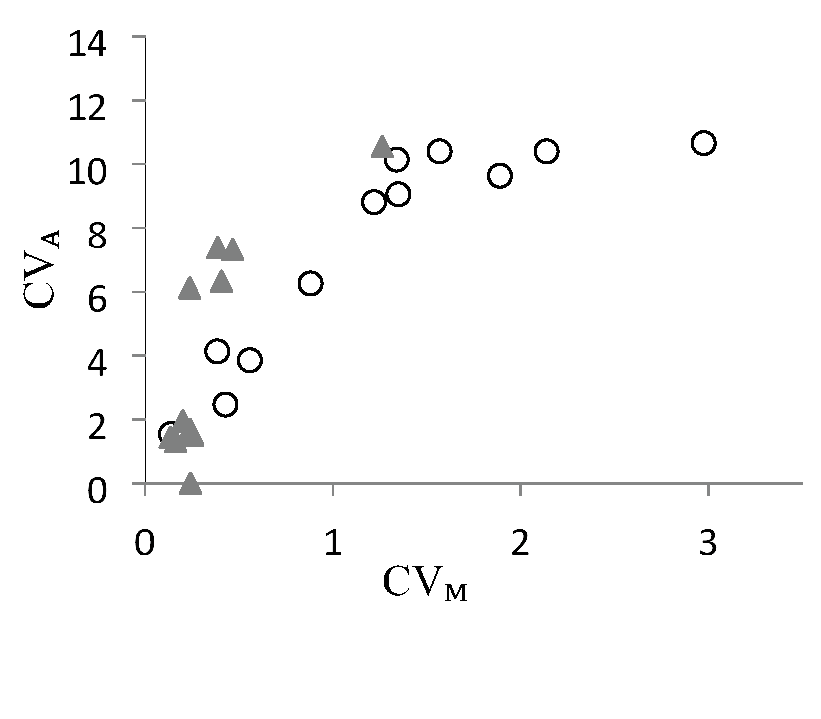
\includegraphics[width=0.65\textwidth]{Chp1_Intro/IntroFig}
\vspace{-1cm}
\caption[Estimates of standing genetic ($CV_A$) against mutational variance ($CV_M$).]{Estimates of standing genetic ($CV_A$) against mutational variance ($CV_M$). There is a strong positive relationship between $CV_M$ and standing genetic variance $CV_A$, suggesting that mutation might be sufficient to explain levels of standing genetic variance. The relationship is plotted separately for life history (open circles) and morphological traits (solid grey triangles) from data taken from \citet{Houl96} and \citet{Houl98}.}
\label{fig:CvaCvm}
\end{figure}
